%*****************************************
\chapter{Stand der Forschung}\label{ch:relatedWork}
%*****************************************

\section{Die Ontologie: SNIK}\label{sec:snik}

Das semantische Netz des Informationsmanagements im Krankenhaus (\ac{snik}) ist eine am \ac{imise} der Universität Leipzig entwickelte,
die Domäne des Informationsmanagements im Krankenhaus betreffende Ontologie \citep{domaene}.
Sie behandelt Wissen über Krankenhausinformationssysteme und deren Management.
Dieses wurde aus drei Lehrbüchern (\citet{bb}, \citet{ob} und \citet{he}) manuell extrahiert und in RDF modelliert.
Desweiteren wurde auch noch ein Interview mit dem Leiter des Informationsmanagements des Universitätsklinkum Leipzigs, Stefan Smers, geführt.

\begin{sidewaysfigure}[htbp!]
\centering
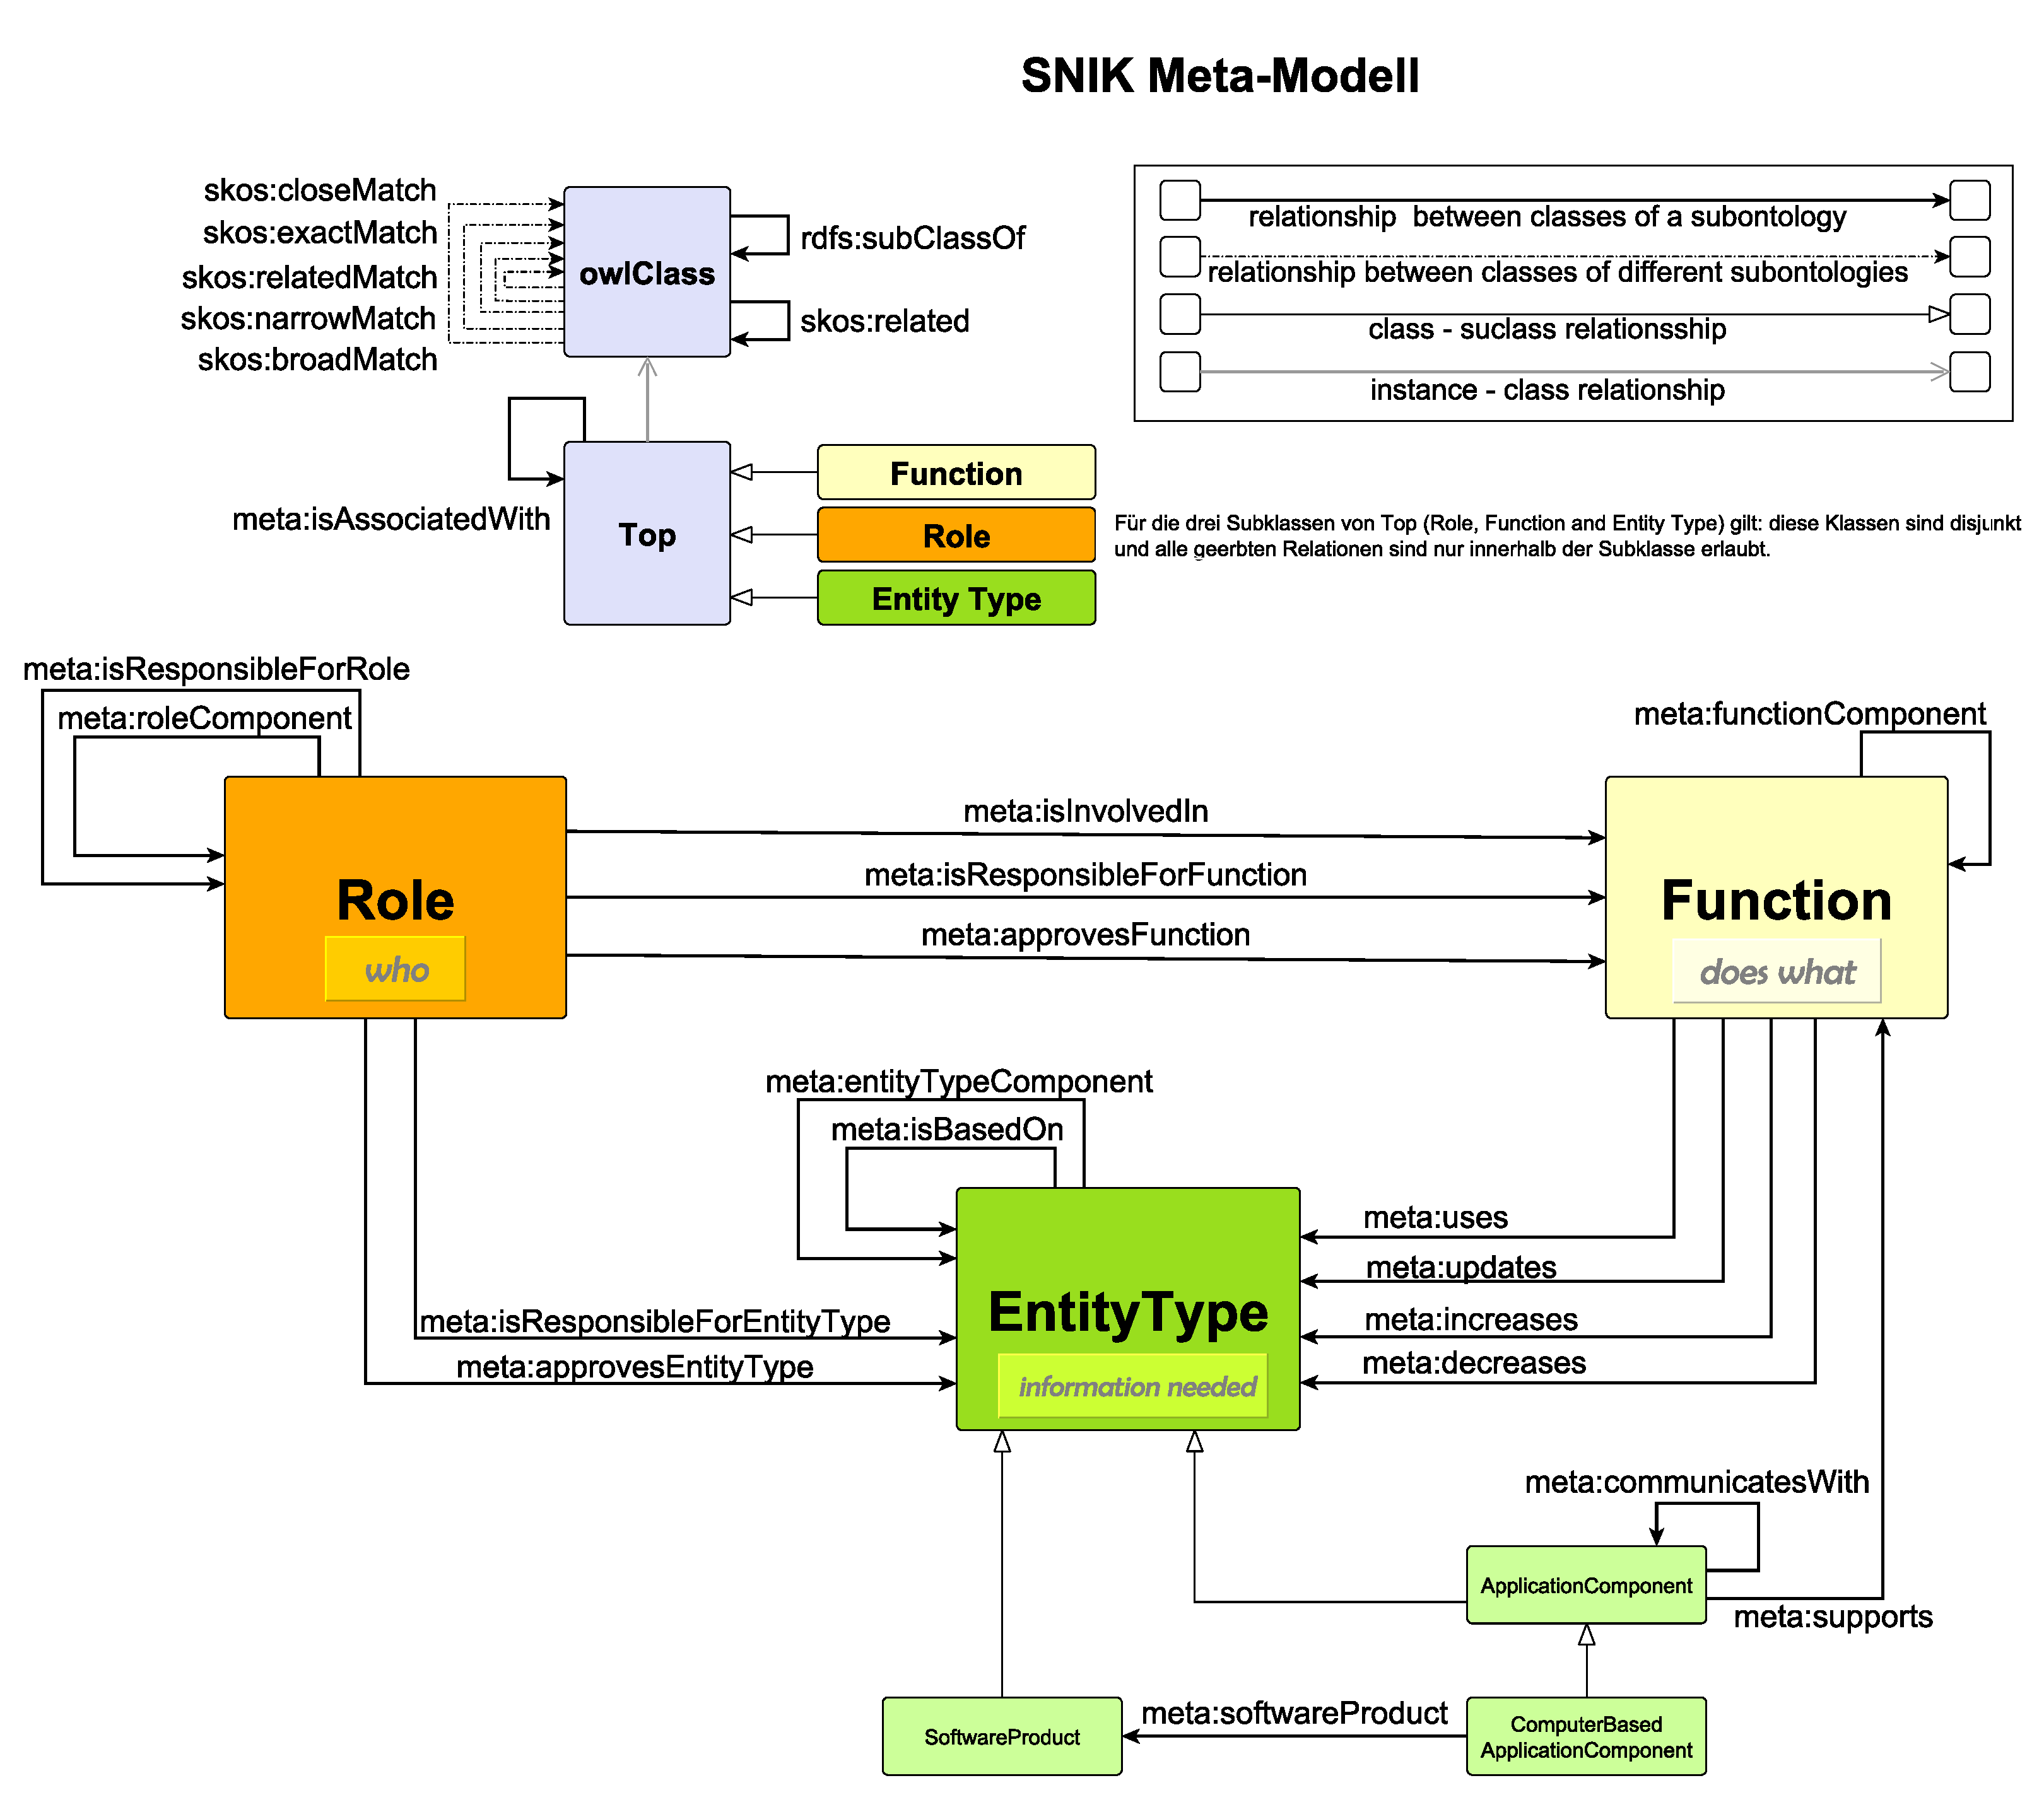
\includegraphics[width=.8\textwidth, height=.9\textheight, keepaspectratio]{Images/snik-metamodel.pdf}
\caption[SNIK Metamodell Version 8]{Das SNIK Metamodell Version 8. Quelle: \url{https://www.snik.eu/public/SNIK_Metamodell_V8.svg}}
\label{fig:snik-metamodel}
\end{sidewaysfigure}

\subsection{\enquote{Eine Ontologie von Ontologien} - Die Architektur SNIKs}

Die einzelnen Bücher liegen jeweils in einer eigenen Subontologie vor.
Es gibt also drei große Teilontologien der \ac{snik}-Ontologie, die die Präfixe \emph{bb}, \emph{ob} und \emph{he} haben.
Das Interview mit dem Leiter des Informationsmanagements befindet sich in der Subontologie mit dem Präfix \emph{ciox}.
Zur Beschreibung der Relationen gibt es eine Ontologie mit dem Präfix \emph{meta}, in der größtenteils Properties stehen.
Diese enthalten dann jeweils Klassen von Individuen, z.B. \aurl{bb}{ChiefInformationOfficer} anstelle von \aurl{ex}{ErikaMustermann}.
Es geht hier nämlich, wie gesagt, um Textbuchwissen und nicht um spezielle Vorgänge \citep{sniktec}.

Die Entitäten\ac{snik}s in einer Subontologie sind, wie in \cref{fig:snik-metamodel} zu sehen, primär nach ihrem Typ gegliedert.
Es gibt Rollen, die eine Person einnehmen kann, wie z.B. \aurl{bb}{ChiefInformationOfficer}, Aufgaben, die eine Rolle hat, wie z.B. \aurl{bb}{HISBudgetPlanning},
und Objekttypen, die Informationen, die für diese Aufgabe benötigt werden, repräsentieren, wie z.B. \aurl{bb}{AnnualITBudget}.
Zwischen diesen gibt es Relationen, die deren Beziehung beschreiben.

Die Subontologien sind theoretisch unabhängig voneinander. Sie sind größtenteils dann verbunden,
wenn sie ähnliche Prinzipien wie ein anderer Punkt einer anderen Subontologie darstellen.
Für das Tripel mit dem Subjekt \aurl{bb}{ChiefInformationOfficer} gibt es das Prädikat \aurl{skos}{closeMatch} mit dem Objekt \aurl{ciox}{ChiefInformationOfficer}.
Es gibt dieses Tripel auch mit diesem als Subjekt und dem anderen als Objekt.
Dies erklärt auch, weshalb auf dem Pfeil zwischen ihnen keine Richtung zu sehen ist.


\subsection{Der SNIK-Graph}

Der \ac{snik}-Graph\footnote{\url{https://www.snik.eu/graph}} ist die Visualisierung von \ac{snik}.
Hier werden die einzelnen Entitäten nach ihrer entsprechenden Subontologie gefärbt visuell dargestellt.
Die beschrifteten Verbindungen bzw. Kanten zwischen den Formen stellen Relationen dar,
welche, wenn sie zwischen zwei Entitäten unterschiedlicher Subontologien verlaufen, keine Richtung haben.
Entitäten werden durch Dreiecke, Quadrate oder Kreise dargestellt und vertreten die verschiedenen Typen.

\section{Stichwortsuche}

Die Stichwortsuche ist wohl mit die am weitesten verbreitete Form, um sich Informationen anzueignen.
Im Gegensatz zu Question Answering werden hier statt ganzen Sätzen nur einzelne Stichwörter eingegeben, womit letztendlich Ergebnisse angezeigt werden.
Das Problem (bzw. der Ansatz) dabei ist nicht unbedingt, den Nutzer zu verstehen, sondern in abertausenden Möglichkeiten die möglichst relevantesten herauszusuchen.
Dazu werden oft Listen, wo die Antwortmöglichkeiten indiziert sind, verwendet.
Stichwortsuche wird nicht nur im \ac{www}, sondern auch in vielen anderen Bereichen eingesetzt.
Manche Question Answering-Systeme verwenden es z.B. auch für bestimmte Module.

\subsection{Elasticsearch}

Elasticsearch\footnote{\url{https://www.elastic.co}} ist ein Open-Source Programm, das einfaches Indizieren, Suchen und Analysieren von Daten ermöglichen soll \citep[S.~8]{elasticsearch}.
Es kann verschiedenste Datentypen durchsuchen, auch Text und Zahlen.
Dazu serialisiert es Dokumente in \ac{json}, einer für die Programmiersprache JavaScript, welche häufig auf Webseiten verwendet wird, lesbare Notation.
In dieser Serialisierung nutzt es einen \emph{invertierten Index}, d.h. es indiziert das Dokument für alle verschieden vorkommenden Wörter \citep{invertedindex}.
Das Wort bzw. die Zeichenkette ist also ein Schlüssel mit den Dokumenten als Wert.
Nehme man z.B. die beiden Sätze \enquote{War is peace.} und \enquote{Freedom is slavery.} \citep[S.~6]{orwell1984} als eigene Dokumente, würde es wie in \cref{tab:invertedindexexample} aussehen.
Das Wort \enquote{is} kommt sowohl in Dokument 1 und 2, das Wort \enquote{war} nur in Satz 1 und das Wort \enquote{freedom} in nur in Satz 2.
Die Zahl nach dem Doppelpunkt zeigt die Position im Satz an, \enquote{peace} ist z.B. an dritter Stelle im ersten Satz.
\begin{table}[h]\centering
  \begin{tabulary}{\textwidth}{rl}
    \toprule
    Schlüssel & Wert(e) \\
    \midrule
    war & 1:1 \\
    is & 1:2,2:2 \\
    peace & 1:3 \\
    freedom & 2:1 \\
    slavery & 2:3 \\
    \bottomrule
  \end{tabulary}
  \caption{Beispiel für invertierte Indizes}
  \label{tab:invertedindexexample}
\end{table}
Elasticsearch verwendet \ac{rest}-\acp{api}, also Programmierschnittstellen, die mittels \ac{http}-Anfragen mit Seiten im \ac{xml}-Format, wie z.B. \ac{html}, kommunizieren.
Mit diesen kann es in der Tabelle nach Informationen suchen.
Das tut es, indem es die Seiten und Positionen, auf denen die eingegebenen Wörter stehen, mithilfe der invertierten Indizes heraussucht.
Je näher die eingegebenen Wörter aneinanderstehen, und je eher die gefundenen Wörter mit den eingegebenen übereinstimmen, desto besser ist das Ergebnis und desto eher wird es angezeigt \citep[S.~23]{elasticsearch}.
Es können auch verschiedene Synonyme und phonetisch ähnlich klingende Wörter ausprobiert werden.

\section{Question Answering-Systeme}

Zur Recherche wurden verschiedene Surveys bezüglich \ac{kbqa} und \ac{cdqa} verwendet.
Außerdem wurden über die Herausforderung \ac{qald} weitere Systeme evaluiert.
Bei \ac{qald} werden Question Answering-Systeme anhand eines Benchmark objektiv bewertet.
Diese fand schon mehrmals statt, die zur Zeit dieser Arbeit aktuelle ist \ac{qald}-9 \citep{qald9}.
In jeder dieser Versionen gibt es unterschiedliche Trainingsdatensätze und Teilnehmer.
Die Teilnehmer müssen zu dem jeweiligen Trainingsdatensatz natürlichsprachige Fragen in \ac{sparql}-Abfragen umformen, also das grundlegende Problem des Question Answerings lösen.
Der jetzige Trainingssatz ist DBpedia.

DBpedia ist eine Wissensbasis, welche aus den Daten Wikipedias besteht.
Es ist das Paradebeispiel für Linked Data und wird häufig zum Training von Question Answering-Programmen genutzt.
Die Daten sind frei verfügbar und in verschiedenen Serialisierungen, wie z.B. im \ac{turtle}-Format, verfügbar.
Über \ac{sparql} können auch direkt online Abfragen getätigt werden.
DBpedia ist außerdem in mehreren Sprachen verfügbar \citep{dbpedia}.

\subsection{Leaderboard}

Das Question Answering-Leaderboard\footnote{\url{https://github.com/KGQA/leaderboard}} \citep{kgqaleaderboard} hat es sich zur Aufgabe gemacht,
dem häufig als sehr uneinheitlich und unübersichtlich \citep{diefenbachkbqa} beschriebenen Feld des \ac{kbqa} eine vereinheitliche Liste mit verfügbaren Question Answering-Systemen zu geben.
Hier sind werden Fragenkataloge wie \ac{qald9} als Benchmarks auf die verschiedenen \ac{kbqa}-Systeme angewendet und die Ergebnisse aufgezeichnet.
Desweiteren sind die 98 Systeme in einer Liste mit dem Namen des Systems, einer Beschreibung und Links zu dem originalen Paper und einer Demonstration,
\ac{rest}-\ac{api} oder dem GitHub-Projekt, falls diese öffentlich verfügbar existieren, ausgestattet.
Dies vereinfacht eine systematische Suche enorm, da viele Systeme schwer auffindbar sind, sowohl in der Dokumentation als auch in Form des implementierten Systems selbst.

\subsection{gAnswer}

gAnswer\footnote{\url{https://github.com/pkumod/gAnswer}} \citep{ganswer2} wurde von dem Wangxuan Institute of Computer Technology entwickelt und arbeitet mit Wissensbasen, um Question Answering-Aufgaben zu lösen.
Hierfür werden die Fragen in Unterfragen aufgespalten und daraus je ein Syntaxbaum erstellt.
Es erzielte durch eine durchdachte Vorbereitung der Trainingsdaten sehr schnelle Trainingszeiten bei niedrigem Speicherverbrauch und hoher Genauigkeit bei der Beantwortung von Fragen.
Das System hat außerdem erkannt, dass man, um effizientes Question Answering zu erreichen, Subgraphen vergleichen kann und somit auch einen neuen Ansatz für die Homonymität hat.
Das bedeutet, dass Wörter, die Verschiedenes bedeuten können, erst nach anfänglicher Lokalisierung des Kontexts betrachtet werden.
Es werden also zuerst Wörter, deren Bedeutung eindeutig ist, betrachtet, und von da aus die kürzeste Verbindung zu einer Bedeutung des fragwürdigen Wortes \citep{ganswerapproach}.
Darauf bauen viele andere Question Answering-Systeme auf.

\subsection{DeepPavlov}
DeepPavlov\footnote{\url{https://www.deeppavlov.ai}} \citep{deeppavlov} ist eine open-source Bibliothek zur Entwicklung von Dialogsystemen.
Es ist in \emph{Models} und \emph{Skills} organisiert.
Das System ist hochdynamisch und auf verschiedenste Aufgaben ausgelegt, vor allem aber Dialogsysteme bzw. Chat Bots.
Für Question Answering gibt es bisher nur Ansätze bezüglich \ac{odqa}.

\subsubsection{Architektur}
Ein \emph{Modell} ist eine in TensorFlow \citep{tensorflow}, einer Schnittstelle für maschinelles Lernen, implementierte Funktion einer \ac{nlp}-Pipeline,
die sowohl ein neuronales Netz als auch ein nichtneuronales oder regelbasiertes System sein kann.
Modelle können auch andere Modelle enthalten.
Eine \emph{Fähigkeit} besteht aus Modellen, jedoch kann sie nur Zeichenketten als Ein-/Ausgabe haben.
Sie werden deshalb häufig im Dialog verwendet.
Die Modelle in Fähigkeiten werden über einen \emph{Chainer} verbunden, der die Konfigurationsdatei einliest und so die Parameter der Modelle festsetzt.
Fähigkeiten und Modelle werden gleich implementiert und unterscheiden sich nur in den unterschiedlichen Ein- und Ausgabemöglichkeiten.
Mehrere Fähigkeiten formen einen \emph{Agenten}, wie in \cref{fig:deeppavlov-architektur} sichtbar ist.
Ein Agent kann die verschiedenen Fähigkeiten, aus denen er besteht, in einer Unterhaltung mit dem Benutzer verwenden und zwischen ihnen wechseln.

\begin{figure}[htbp!]
\centering
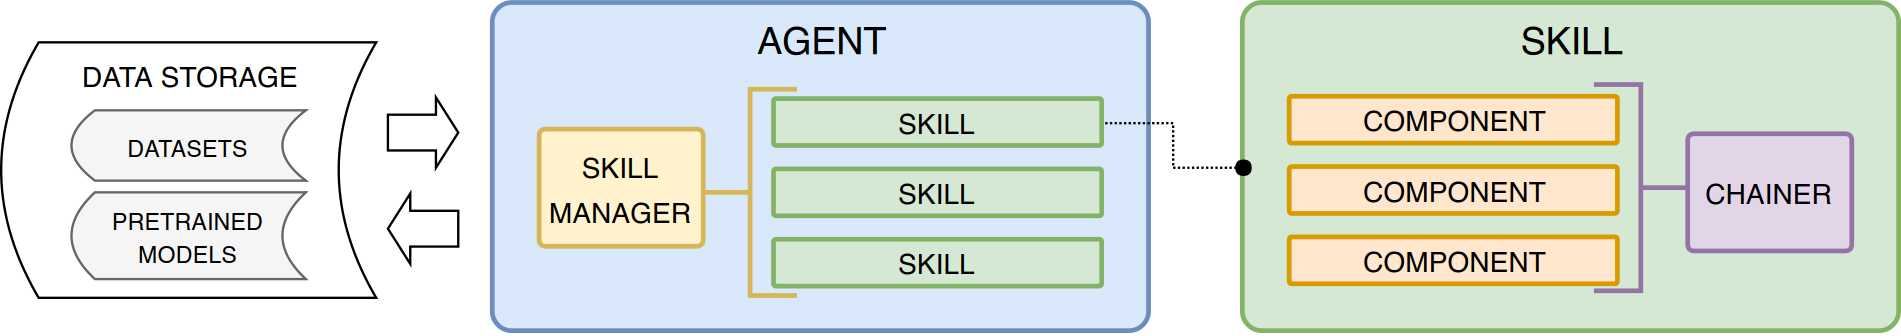
\includegraphics[width=\textwidth, height=\textheight, keepaspectratio]{Images/DeepPavlovArchitecture.png}
\caption[DeepPavlov Architektur]{Die Architektur von DeepPavlov. Quelle: \citet{deeppavlov}}
\label{fig:deeppavlov-architektur}
\end{figure}

\subsection{TeBaQA}

TeBaQA\footnote{\url{https://github.com/dice-group/TeBaQA}} \citep{tebaqa} wird von der Forschungsgruppe DICE an der Universität Paderborn entwickelt.
Es basiert darauf, Fragen anhand ihrer Struktur zu gruppieren.
Dabei werden isomorphe \ac{sparql}-Anfragen, d.h. Anfragen gleicher Struktur, einer Vorlage zugeordnet.
Somit können schnellere Antwortzeiten ermöglicht werden.
Mit Struktur ist die Form der RDF-Relationen gemeint, wobei diese als Kanten zwischen den verschiedenen Informationen gesehen werden.

\subsubsection{Architektur}

TeBaQA wird in fünf Phasen aufgebaut.
In der ersten Phase, dem \emph{Preprocessing} (Vorverarbeitung), werden Wörter, die keinen semantischen Wert und somit keine Information tragen, entfernt.
Das können etwa Artikel sein, wodurch die Assoziation der Wörter mit vielen unzusammenhängenden Einträgen vermieden wird.
Damit solche Wörter, die auch Teil der Entitäten, wie z.B. \enquote{the} in \aurl{bb}{AdaptabilityOfTheHIS},
nicht auch dort herausgefiltert werden, müssen die Wörter gruppiert und die resultierenden Gruppen überprüft werden.
Die zweite Phase befasst sich mit der Isomorphie der Abfragegraphen und der Vorlagenklassifizierung.
Hier wird die zu nutzende Vorlage der Abfrage identifiziert und darüber Eigenschaften der Frage, also z.B. Fragewörter,
Anzahl der Nomen, mindestens benötigte Tripel oder ob Personen referenziert werden.
Die Einordnung in eine Vorlage geschieht, wie vorher schon erwähnt, über die Struktur der \ac{sparql}-Abfrage.
Die Reihenfolge der Elemente wird hierbei nicht betrachtet.
Beispielsweise resultiert die Frage \enquote{Wofür ist die Leiterin des Informationsmanagements zuständig?}
in einer Abfrage mit der gleichen Struktur wie die Abfrage der Frage \enquote{Wovon wird 3LGM² erzeigt?}.
Die \ac{sparql}-Abfrage könnte bei beiden so aussehen, bei der ersten Abfrage wäre das Individuum im Subjekt \aurl{bb}{ChiefInformationOfficer} und das Prädikat \aurl{meta}{isResponsibleForEntityType},
bei der zweiten Frage das Subjekt \aurl{bb}{3LGM2} und das Prädikat \aurl{meta}{isBasedOn}.
\begin{lstlisting}
  PREFIX bb: <http://snik.eu/ontology/bb/>
  PREFIX meta: <http://snik.eu/ontology/meta/>
  SELECT ?uri
  WHERE
    { <Subjekt> <Prädikat> ?uri }
\end{lstlisting}
Das Ergebnis, ?uri, ist \aurl{bb}{AnnualITBudget} bzw. \aurl{bb}{UmlClassDiagram}, also beide Male eine Entität.
Wenn die Vorlage zugeordnet wurde, können Eigenschaften der Frage, wie oben beschrieben, in einen Vektor getan und weiterverwendet werden.
Im dritten Schritt werden speziell referenzierte Individuen und Klassen identifiziert, also nicht nur wie im 2. Schritt generelle Informationen über den Inhalt der Frage.
Hier werden auch verschiedene Synonyme der eingegebenen Wörter untersucht, um ein möglichst genaues Ergebnis zu erreichen.
Im vierten Schritt wird die Anfrage geschrieben, also die Vorlage gefüllt und eventuelle Parameter gesetzt.
Die letzte Phase behandelt das Auswählen der Lösung, die dem Nutzer übergeben werden soll.
Dazu wird wieder auf das Fragewort geblickt, um herauszufinden, in was für einer Form, z.B. einem Datum, der Nutzer die Antwort erwartet.
Das erste Substantiv nach dem Fragewort wird überprüft, um den Numerus der Frage zu erkennen.
Desweiteren werden die Lösungskandidaten auf ihre Ähnlichkeit mit der Frage überprüft, woraus eine Bewertung und letztendlich die zu präsentierende Antwort berechnet wird.

\subsection{Qanswer KG}

QAnswer KG \citep{qanswer} ist ein an der Universität Saint-Étienne entwickeltes Question Answering-System,
das vor allem das von \citet{diefenbachkbqa} genannte Problem der fehlenden Portabilität in diesem Feld lösen soll:
Viele Systeme wurden als Forschungsprojekt für Benchmarks wie \ac{qald}-9 geschrieben und sind deshalb nur mit großen Ontologien wie DBpedia oder Wikidata kompatibel.
Hier ist es jedoch möglich, auf einer Website einfach eigene Daten hochzuladen und dort Question Answering zu betreiben.
Die Modelle müssen aber noch auf die Fragen trainiert werden, das vortrainierte Modell soll nur Sprache an sich verstehen können und nicht den speziellen Datensatz.
Alles in allem kann man dennoch sagen, dass das System vergleichsweise sehr leicht zu verwenden ist.
Selbst ein fast nicht trainiertes System bietet oft noch akzeptable Antworten.
Es ist leider nicht open-source, steht online\footnote{Demo: \url{https://qanswer-frontend.univ-st-etienne.fr}\\Website: \url{https://www.qanswer.eu}} aber frei zur Verfügung und wird es nach Nachfrage auch für mindestens die nächsten zwei Jahre noch bleiben.

\subsubsection{Architektur}

\begin{figure}%[htbp!]
\centering

\includegraphics[width=\textwidth, height=\textheight, keepaspectratio]{Images/QAnswerWorkflow.png}
\caption[QAnswer KG Arbeitsablauf]{Arbeitsablauf von QAnswer KG \citep{qanswer}.}
\label{fig:qanswerworkflow}
\end{figure}

QAnswer KG beantwortet eine Frage in vier Schritten, die in \cref{fig:qanswerworkflow} dargestellt sind.
Zuerst werden alle sogenannten \emph{N-Gramme} gebildet, d.h. alle möglichen Kombinationen von aufeinanderfolgenden Wörtern mit der maximalen Länge n.
Die maximale Länge hier ist die Anzahl der Wörter im Satz, d.h. der Satz selbst ist auch ein N-Gramm.
Wenn man zum Beispiel die Frage \enquote{Is war peace?} stellt,
sucht das Programm für jedes Wort sowie für die Kombinationen \enquote{is war}, \enquote{war peace} und \enquote{is war peace}
mithilfe des auf natürliche Sprache vortrainierten Modells die am ehesten passenden Werte im Datensatz heraus.
Dabei werden normalerweise auch viele falsche Ressourcen ausgewählt, da besonders bei längeren Fragen viele N-Gramme existieren.
Danach werden aus all diesen Werten alle möglichen \ac{sparql}-Anfragen erstellt.
Dabei werden auch die falschen Interpretationen weitergeführt, jedoch sollte auch die richtige dabei sein.
Deshalb müssen die Abfragen im dritten Schritt bewertet werden.
Dazu werden mithilfe von verschiedenen Parametern und einer künstlichen Intelligenz die Kandidaten evaluiert.
Parameter sind etwa die Anzahl der in der Abfrage verwendeten mit einer Ressource assoziierten Wörter verglichen mit der Anzahl der Wörter in der Frage,
oder die Ähnlichkeit der Label mit den entsprechend ausgewählten Wörtern.
Label werden meist über das \ac{rdf}-Property \aurl{rdfs}{label} festgelegt.
Dadurch soll die Interpretation, die der Intention der Frage am nächsten kommt, am höchsten gewertet sein.
Diese wird im letzten Schritt analysiert und es wird entschieden, ob es die richtige Antwort ist.
Damit wird ein \enquote{confidence score}, zu Deutsch etwa \enquote{Vertrauenswert}, erstellt.
Sollte dieser unter 50\% liegen, gilt die Frage als falsch beantwortet.
Sie wird jedoch trotzdem ausgegeben.

\subsubsection{Vorteile, Grenzen und Probleme}

Im Gegensatz zu anderen Ansätzen verwendet QAnswer KG kein herkömmliches \ac{nlp}, wo auf sprachliche Eigenschaften acht gegeben wird, wie man bei TeBaQA gut sehen kann.
Dies führt dazu, dass auch Stichwortsuche und Fragen mit fragwürdiger Grammatik und teils auch Rechtschreibung beantwortet werden können, was in der Praxis sehr hilfreich ist.
Nicht jede die Applikation benutzende Person ist in diesen Bereichen sicher, besonders, wenn das Programm auch im öffentlichen Bereich einsetzbar sein soll.
Ein weiterer ausschlaggebender Punkt ist, dass dadurch Fragen in verschiedenen Sprachen gestellt werden können, solange die Ontologie in diesen verfügbar ist.
Außerdem können verschiedene Ontologien gleichzeitig durchsucht werden, was insbesondere in Zeiten von Linked Open Data hilfreich ist.
Systeme wie gAnswer benötigen die Daten auch in einer speziellen Form, um sie verarbeiten zu können, hier reichen die \ac{rdf}-Daten aus.
Das hilft den Entwicklern, die dieses System verwenden wollen, weiter, indem es den Entwicklungsaufwand senkt..

Diese die Semantik des Satzes nicht beachtende Methode bringt allerdings auch Nachteile mit sich.
Der größte ist wohl, dass das Wissen sich in einer bestimmten Form befinden muss.
Es müssen \aurl{rdfs}{label}s o.ä. verwendet werden, anderes wird nicht erkannt.
Desweiteren müssen die Label eine Annotation, die deren Sprache bestimmt, besitzen, also zum Beispiel \texttt{\enquote{Chief Information Officer}@en, \enquote{Leiter des Informationsmanagements}@de}
für das Label vom \aurl{bb}{ChiefInformationOfficer}.
Bei \ac{snik} und den meisten anderen Wissensbasen ist das allerdings kein Problem, da sie es bereits besitzen.
Das zieht allerdings auch mit sich, dass andere Informationen, die in der Wissensbasis existieren, aber nicht im Label gespeichert sind, nicht mit betrachtet werden.
Eine weitere bedeutende Grenze ist die Limitierung der Komplexität der \ac{sparql}-Abfrage auf maximal drei Tripel, sodass besonders komplexe Fragen mit kompliziertem Muster nicht beantwortet werden können.
In der Praxis sollten diese allerdings für die meisten Fragen ausreichen.
Gäbe es diese Limitation nicht, würde die Beantwortung längerer Fragen aufgrund des Versuches, aus den N-Grammen zu komplexe Muster zu erstellen,
vermutlich mit einer geringeren Genauigkeit der Ergebnisse und einer langsameren Geschwindigkeit ausfallen.

QAnswer KG kann, wie man an Benchmarks sieht, mit den bisher existierenden Systemen mithalten, ist jedoch in der Intuitivität und Portabilität weit über ihnen.
Mit Training kann auch eine sehr hohe Genauigkeit erzielt werden.
